\documentclass[tikz,border=2pt]{standalone}
% Preámbulo común de los diagramas TikZ (misma paleta y letra que las notas)
\usepackage[T1]{fontenc}\usepackage[utf8]{inputenc}
\usepackage{libertinus}\usepackage{libertinust1math}
\usepackage[defaultsans,scale=0.92]{lato}
\usepackage{amsmath,amssymb,bm}
\usepackage{tikz}\usetikzlibrary{calc,positioning,arrows.meta,shapes.geometric,decorations.pathreplacing,decorations.pathmorphing,fit,backgrounds}
\definecolor{snlazul}{HTML}{1E5AA8}\definecolor{snlnoche}{HTML}{14213D}\definecolor{snlvioleta}{HTML}{6C4AB6}
\definecolor{snlcoral}{HTML}{D1495B}\definecolor{snlambar}{HTML}{E09F3E}\definecolor{snlverde}{HTML}{2A9D8F}
\definecolor{snlteal}{HTML}{0F7173}\definecolor{snlgris}{HTML}{5C677D}\definecolor{snlfondo}{HTML}{F4F6FA}
\tikzset{>={Stealth[length=2.2mm]},
  bloque/.style={draw=#1,fill=#1!8,thick,rounded corners=2pt,minimum height=11mm,minimum width=20mm,align=center,font=\small},
  bloque/.default=snlazul,
  suma/.style={draw=snlnoche,thick,circle,inner sep=0pt,minimum size=5mm},
  flecha/.style={->,thick,draw=snlnoche},
  etq/.style={font=\small,text=snlnoche},
  nota/.style={font=\footnotesize\sffamily,text=snlgris,align=center}}

\usepackage[siunitx,american]{circuitikz}
\begin{document}
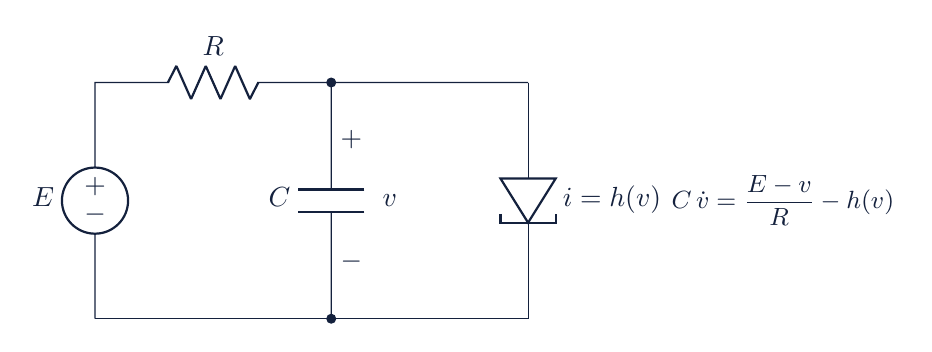
\begin{tikzpicture}[color=snlnoche]
 \draw (0,0) to[V,l=$E$,invert] (0,3) to[R,l=$R$] (3,3) -- (5.5,3);
 \draw (3,3) to[C,l_=$C$,v^>=$v$] (3,0);
 \draw (5.5,3) to[tDo,l={$i=h(v)$}] (5.5,0);
 \draw (0,0) -- (5.5,0);
 \draw (3,3) node[circ]{} (3,0) node[circ]{};
 \node[etq,anchor=west] at (7.2,1.5) {$C\,\dot v=\dfrac{E-v}{R}-h(v)$};
\end{tikzpicture}
\end{document}
